\documentclass{article}
\usepackage[utf8]{inputenc}
\usepackage[polish]{babel}
\usepackage[T1]{fontenc}
\usepackage{booktabs}
\usepackage{graphicx}
\usepackage{amsmath}
\usepackage{siunitx}
\usepackage{geometry}
\usepackage{float}

\geometry{margin=1in}

\title{Analiza stabilności algorytmów sumowania w zależności od precyzji typu danych}
\author{Artur Radwański}
\date{12 marca 2026}

\begin{document}

\maketitle

\section{Środowisko}
\begin{itemize}
    \item System operacyjny: Linux 6.17.9-arch1-1
    \item Procesor: Intel Core i5-7200U
    \item Język programowania: c++ 
    \item Wersja kompilatora: gcc version 15.2.1 20260209 (GCC)
\end{itemize}

\section{Algorytm sumacyjny Kahana}

Algorytm Kahana pozwala na znaczną redukcję błędu zaokrągleń podczas sumowania ciągu liczb zmiennoprzecinkowych. Dla każdego elementu wejściowego $x_i$, przy założeniu wartości początkowych $s_0 = 0$ oraz $c_0 = 0$ (poprawka), wykonuje się następujące kroki:

\begin{enumerate}
    \item \textbf{Obliczenie poprawionej wartości:}
    \[ y_i = x_i - c_{i-1} \]
    \textit{Od bieżącego elementu odejmujemy zakumulowany błąd z poprzedniej iteracji.}

    \item \textbf{Wyznaczenie sumy tymczasowej:}
    \[ t_i = s_{i-1} + y_i \]
    \textit{W tym kroku następuje właściwa operacja dodawania, w której mniejsze bity $y_i$ mogą zostać odcięte.}

    \item \textbf{Obliczenie nowej poprawki:}
    \[ c_i = (t_i - s_{i-1}) - y_i \]
    \textit{Obliczamy różnicę między tym, co faktycznie zostało dodane do sumy $(t_i - s_{i-1})$, a wartością, którą zamierzaliśmy dodać ($y_i$).}

    \item \textbf{Aktualizacja sumy głównej:}
    \[ s_i = t_i \]
\end{enumerate}

Dzięki takiemu podejściu, błąd odcięty w kroku 2. zostaje "odrodzony" w zmiennej $c_i$ i uwzględniony (z przeciwnym znakiem) w kolejnej iteracji, co pozwala zachować precyzję zbliżoną do typów o wyższej rozdzielczości (np. \texttt{double} dla danych typu \texttt{float}).

\section{Wyniki eksperymentu}

W tabeli \ref{tabela-wyniki} zestawiono wyniki sumowania $1.0$ oraz $10^6$ składników o wartości $10^{-6}$ dla trzech różnych typów precyzji.

\begin{table}[h!]
\centering
\begin{tabular}{@{}lccc@{}}
\toprule
\textbf{Algorytm} & \textbf{float} (32-bit) & \textbf{double} (64-bit) & \textbf{long double} (80-bit) \\ \midrule
Wartość oczekiwana & 2.0000000000 & 2.0000000000 & 2.0000000000 \\ \midrule
Dodawanie naturalne & 1.9536743164 & 1.9999999999 & 2.0000000000 \\
Suma Kahana & 2.0000000000 & 2.0000000000 & 2.0000000000 \\
Sumowanie (HeapSort) & 2.0090389252 & 2.0000000000 & 2.0000000000 \\ \bottomrule
\end{tabular}
\caption{Porównanie wyników sumowania w zależności od typu danych.}
\label{tabela-wyniki}
\end{table}

\section{Analiza błędów i uwarunkowanie zadania}

\subsection{Uwarunkowanie zadania}
Zadanie sumowania liczb o drastycznie różnych rzędach wielkości ($1.0$ oraz $10^{-6}$) jest klasycznym przykładem \textbf{złego uwarunkowania numerycznego}. W arytmetyce zmiennoprzecinkowej IEEE 754, aby dodać dwie liczby, ich wykładniki muszą zostać wyrównane, co powoduje przesunięcie mantysy mniejszej liczby w prawo.

\subsection{Analiza wyników dla typu \texttt{float}}
\begin{itemize}
    \item \textbf{Dodawanie naturalne (1.9536):} Wynik jest mniejszy od oczekiwanego z powodu zjawiska \textbf{absorpcji}. Gdy suma częściowa rośnie, mantysa liczby $10^{-6}$ traci najmłodsze bity. W pewnym momencie składnik staje się "za mały", by zmienić wartość sumy, co generuje stały błąd systematyczny.
    \item \textbf{Algorytm Kahana (2.0000):} Wykazuje najwyższą stabilność. Wykorzystuje zmienną poprawki $c$ do przechowywania utraconych bitów (ang. \textit{lost low-order bits}) i uwzględnia je w następnej iteracji, co pozwala na osiągnięcie precyzji maszynowej bez sortowania.
    \item \textbf{HeapSort (2.0090):} Wynik powyżej 2.0 sugeruje błąd typu overflow przy arytmetyce float.
\end{itemize}

\subsection{Wpływ precyzji (\texttt{double} i \texttt{long double})}
Przejście na \texttt{double} zwiększa mantysę z 24 do 53 bitów. Błąd absorpcji dla $10^6$ operacji przesuwa się poza zakres widoczny w standardowym wypisywaniu (pojawia się dopiero jako $1.9999999999$). Dla \texttt{long double} precyzja jest na tyle wysoka, że błąd zaokrągleń dla tej skali danych jest nieobserwowalny.

\begin{figure}[H]
  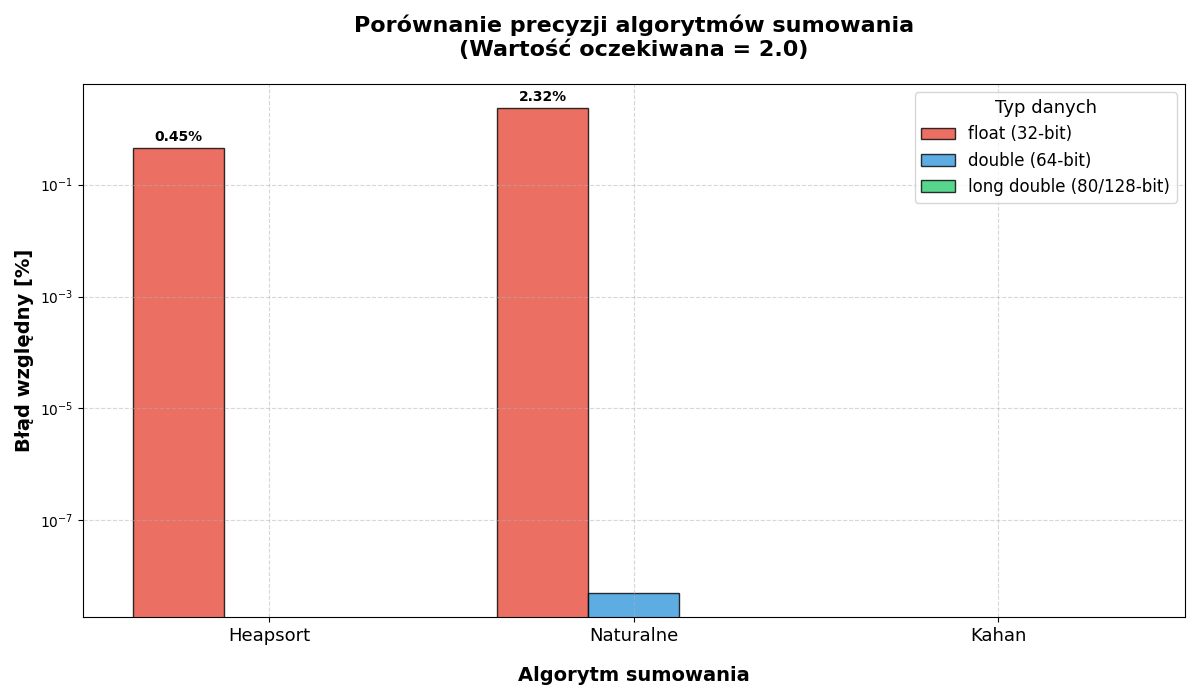
\includegraphics[width=\linewidth]{wykres.png}
  \caption{Wykres błędu względnego otrzymanego wyniku w porównaniu do wyniku teoretycznego}
  \label{fig:boat1}
\end{figure}

\section{Analiza czasu wykonywania}
Analiza czasu wykonywania wskazuje na istotne różnice w koszcie operacji zmiennoprzecinkowych oraz dostępu do pamięci, zwłaszcza w przypadku long double.

\begin{table}[h!]
\centering
\begin{tabular}{@{}lccc@{}}
\toprule
\textbf{Algorytm} & \textbf{float} [s] & \textbf{double} [s] & \textbf{long double} [s] \\ \midrule
Dodawanie naturalne & 0.003466 & 0.003520 & 0.003962 \\
Suma Kahana         & 0.011358 & 0.011532 & 0.016004 \\
Sumowanie (HeapSort)& 0.026127 & 0.027380 & 0.045618 \\ \bottomrule
\end{tabular}
\caption{Czas wykonania algorytmów dla $10^6$ elementów [sekundy].}
\end{table}

\subsection{Interpretacja wyników wydajnościowych}
\begin{enumerate}
    \item \textbf{Efektywność sumowania naturalnego:} Jest to najszybsza metoda, ponieważ procesor wykonuje tylko jedną operację dodawania na element ($sum += x$). Bardzo niski czas dla \texttt{double} sugeruje optymalne wykorzystanie instrukcji wektorowych (SIMD) przez kompilator.
    \item \textbf{Koszt Algorytmu Kahana:} Kahan jest około $2$-$3$ razy wolniejszy od sumowania naturalnego. Wynika to z faktu, że na każdy element tablicy przypadają cztery operacje zmiennoprzecinkowe, które tworzą łańcuch zależności (ang. \textit{dependency chain}), uniemożliwiając pełne równoległe przetwarzanie wewnątrz rdzenia.
    \item \textbf{Złożoność HeapSort:} Jest to metoda zdecydowanie najwolniejsza ($O(n \log n)$). Co ciekawe, czas dla \texttt{double} ($0.16$\,s) jest znacznie wyższy niż dla \texttt{float}, co wynika z większego obciążenia szyny pamięci oraz faktu, że dane typu \texttt{double} zajmują dwa razy więcej miejsca w Cache L2/L3.
\end{enumerate}
\end{document}